\documentclass[12pt, twoside]{article}
% \documentclass[12pt, twoside]{article}
\usepackage[letterpaper, margin=1in, headsep=0.2in]{geometry}
\setlength{\headheight}{0.6in}
%\usepackage[english]{babel}
\usepackage[utf8]{inputenc}
\usepackage{microtype}
\usepackage{amsmath}
\usepackage{amssymb}
%\usepackage{amsfonts}
\usepackage[nomessages]{fp} %\FPeval{\var-name}{2*sin(pi/6)}
\usepackage{siunitx} %units in math. eg 20\milli\meter
\usepackage{yhmath} % for arcs, overparenth command
\usepackage{tikz} %graphics
\usetikzlibrary{quotes, angles, arrows, arrows.meta}
\usepackage{graphicx} %consider setting \graphicspath{{images/}}
\usepackage{parskip} %no paragraph indent
\usepackage{enumitem}
\usepackage{multicol}
\usepackage{venndiagram}

\usepackage{fancyhdr}
\pagestyle{fancy}
\fancyhf{}
\renewcommand{\headrulewidth}{0pt} % disable the underline of the header
\raggedbottom
\hfuzz=2mm %suppresses overfull box warnings

\usepackage{hyperref}
\usepackage{float}

\title{Algebra 2}
\author{Chris Huson}
\date{November 2023}

\fancyhead[LE]{\thepage}
\fancyhead[RO]{\thepage \\ Name: \hspace{4cm} \,\\}
\fancyhead[LO]{BECA / Huson / Algebra 2: Polynomials \\* 17 November 2023}

\begin{document}

\subsubsection*{2.12 Trimester Exam: Polynomial functions}
\begin{enumerate}

\subsubsection*{A1-A.APR.1 Add, subtract, and multiply polynomials}
\item Evaluate each polynomial for the given value of $x$.
\begin{multicols}{2}
    \begin{enumerate}[itemsep=1cm]
        \item $f(x)=x^3+2x^2-7x+8$\\[0.25cm] 
        $f(0) = $
        \item $g(x)=5x^2-3x+11$ \\[0.25cm] 
        $g(1) = $
    \end{enumerate}
    \end{multicols} \vspace{1cm}

\item Find the sum in standard form $(3x^3+2x^2-9x+1)+(x^3+4x^2-x-7)$ \vspace{2.5cm}

\item Find the difference $f(x)-g(x)$ as a polynomial in standard form, with \\[0.25cm]
    $f(x)=7x^3-3x+5$ and $g(x)=x^3-2x^2-1$. \vspace{3cm}

\item Multiply the two polynomials $f(x)=2x^2+4$ and $g(x)=x^2-3x+5$. First complete the grid and then collect terms to find the product as a polynomial in standard form. \\[0.25cm]
\renewcommand{\arraystretch}{2}
\begin{tabular}{|p{1cm}|p{3cm}|p{3cm}|p{3cm}|}
    \hline
     & $x^2$ & $-3x$ & $+5$ \\
    \hline
    $2x^2$ &  & & \\
    \hline
    $+4$ &  & & \\
    \hline
\end{tabular} \vspace{3cm}

\newpage
\subsubsection*{A1-A.APR.3 Identify zeros of polynomials when factorizations are available.}
\item Select all solutions to the equation $(x-6)(2x+6)=0$.
    \begin{multicols}{3}
    \begin{enumerate}
        \item $x= -3$
        \item $x= 6$
        \item $x=\frac{1}{6}$
        \item $x= -\frac{1}{3}$
        \item $x= -6$
        \item $x=-\frac{6}{2}$
    \end{enumerate}
    \end{multicols}

\item Select all of the expressions that are equivalent to $x^2-x-6$.
    \begin{multicols}{2}
    \begin{enumerate}
        \item $(x-2)(x+3)$
        \item $(x-2)(x-3)$ 
        \item $(x-1)(x+6)$ 
        \item $(x+2)(x-3)$ 
        \item $(x+2)(x+3)$ 
        \item $x^2+x+6$
    \end{enumerate} 
    \end{multicols}

\item Write down the solutions to the equation $x(x-5)(3x-9)(x+1)=0$. \vspace{2cm}

\item Identify all of the polynomials having zeros of $x = 0, -2, 4, 7$.
\begin{multicols}{2}
    \begin{enumerate}
        \item $2(x-2)(x+4)(x+7)$
        \item $2x(x-2)(x+4)(x+7)$ 
        \item $x(x-2)(x+4)(x+7)$ 
        \item $2(x+2)(x-4)(x-7)$ 
        \item $2x(x+2)(x-4)(x-7)$
        \item $x(x+2)(x-4)(x-7)$ 
    \end{enumerate} 
    \end{multicols}

\subsubsection*{A2-F.IF.7c Graph polynomials, identify zeros, end behavior}
\item Here is the graph of a quadratic function. Which of the following could be its equation?
\begin{multicols}{2}
    \begin{enumerate}
        \item $y=(x+3)(x-4)$
        \item $y=(x-3)(x+4)$
        \item $y=(x+3)(x+4)$
        \item $y=(x-3)(x-4)$
    \end{enumerate} \vspace{1cm} \;

    \columnbreak
    \begin{tikzpicture}[xscale=0.7, yscale=0.3]
        \draw [thick, ->] (-4.2,0) -- (5.4,0) node [above] {$x$};
        \draw [thick, ->] (0,-13.2)--(0,8.5) node [right] {$y$};
        \foreach \x in {-4,...,-1,1,2,...,4} \draw (\x cm,10pt)--(\x cm,-10pt) node[below] {$\x$};
        \draw [thick, <->,smooth,samples=20,domain=-3.5:4.5] plot(\x,\x*\x-\x-12);
    \end{tikzpicture}
    \end{multicols}

\newpage
\item Given $f(x) = x(x-3)(x+7)(x+11)$. Select the true statements.
    \begin{enumerate}
    \item $f(3)=0$
    \item $f$ is a 4th degree polynomial.
    \item One of the roots of $f$ is 7.
    \item An ordered pair satisfying the equation is $(-11,0)$
    \item $f(0)=0$
    \end{enumerate}

\item Below is a graph of the polynomial $f(x)$. 
\begin{multicols}{2}
    What is the degree of the function?\\[1cm]
    Which of the following could be its equation?
    \begin{enumerate}
        \item $f(x)=(x+2)(x-3)^2$
        \item $f(x)=(x-2)(x+3)^2$
        \item $f(x)=(x+3)(x-2)^2$
        \item $f(x)=(x-3)(x+2)^2$
    \end{enumerate} \vspace{1cm} \;

    \columnbreak
    \begin{tikzpicture}[xscale=0.7, yscale=0.7]
        \draw[lightgray,very thin] (-4,-5) grid (4,4);
        \draw [thick, ->] (-4.2,0) -- (4.8,0) node [above] {$x$};
        \draw [thick, ->] (0,-5.2)--(0,4.5) node [right] {$y$};
        \foreach \x in {-4,4} \draw (\x cm,-10pt) -- (\x cm,10pt) node[above] {$\x$};
        \draw (5pt,4 cm) -- (-5pt,4 cm) node[left] {$20$};
        \draw [thick, <->,smooth,samples=20,domain=-4.2:2.4] plot(\x,{0.2*(\x-2)*(\x+3)^2});
    \end{tikzpicture}
\end{multicols}

\item The polynomial $g(x)=-x^4-3x^3+9x^2+27x$ is graphed below. 
\begin{multicols}{2}
    \begin{enumerate}[itemsep=0.5cm]
        \item What is the leading coefficient?
        \item What are roots of the function?
        \item What factor has a multiplicity of 2?
        \item Write down the $y$-intercept as an ordered pair.
        \item What is the end behavior?
    \end{enumerate} \vspace{1cm} \;

    \columnbreak

    \begin{tikzpicture}[xscale=0.7, yscale=0.7]
        \draw[lightgray,very thin] (-4,-4) grid (4,5);
        \draw [thick, ->] (-4.2,0) -- (4.4,0) node [above] {$x$};
        \draw [thick, ->] (0,-4.2)--(0,5.5) node [right] {$y$};
        \foreach \x in {-4,4} \draw (\x cm,5pt) -- (\x cm,-5pt) node[below] {$\x$};
        \draw (5pt,5 cm) -- (-5pt,5 cm) node[left] {$50$};
        \draw [thick, <->,smooth,samples=20,domain=-4.:3.3] plot(\x,{-0.1*(\x)*(\x-3)*(\x+3)^2});
    \end{tikzpicture}
\end{multicols}

\newpage
\subsubsection*{A2-F.BF.2 Write arithmetic and geometric sequences with recursive formulas}
\item Write a recursive formula for each sequence. Use subscript notation.
    \begin{multicols}{2}
    \begin{enumerate}
        \item $1, 3, 5, 7, 9, \dots$
        \item $\displaystyle +\frac{3}{1}, -\frac{3}{2}, +\frac{3}{4}, -\frac{3}{8},  \dots$ 
    \end{enumerate}
    \end{multicols} \vspace{2cm}

\item Write a recursive definition of the arithmetic sequence $a$. \\[0.5cm]
\renewcommand{\arraystretch}{1.5}
\begin{tabular}{|c|c|}
\hline
$n$ & $a_n$ \\
\hline
$1$ & $8$ \\
$2$ & $-2$ \\
$3$ & $-12$ \\
\hline
\end{tabular}

\item Write a recursive definition of the geometric sequence $a_1 = 1$, \ldots, $a_3 = 9$, $a_4 = 27, \ldots$  \vspace{3cm}

\item The polynomial function $A$, shown below, is used to model the value of an investment account. Three deposits were made which earned interest annually.  $$A(x)=300x^4+100x^3+250x^2$$ 
    \begin{enumerate}[itemsep=1cm]
        \item How much was the first deposit, and how long ago was it made? \vspace{1cm}
        \item If the polynomial is evaluated for $x = 1.06$, what interest rate would that represent \emph{as a percentage}?
        \item Find the value of $A(1.06)$ to the \emph{nearest cent}. \vspace{2cm}
    \end{enumerate}

\end{enumerate}
\end{document}